\def\lecturenumber{12}
\documentclass[11pt,a4paper]{article}
\usepackage[T1]{fontenc}
\usepackage[utf8]{inputenc}
\usepackage{lmodern}
\usepackage[margin=19mm,top=21mm,bottom=21mm,headheight=15pt]{geometry}
\usepackage{amsmath,amssymb,booktabs,array,graphicx,microtype}
\usepackage[dvipsnames]{xcolor}
\usepackage{enumitem,fancyhdr,listings,tcolorbox}
\usepackage[colorlinks=true,linkcolor=MidnightBlue,urlcolor=MidnightBlue]{hyperref}
\definecolor{courseblue}{HTML}{164B69}
\definecolor{pale}{HTML}{F0F5F7}
\pagestyle{fancy}
\fancyhf{}
\fancyhead[L]{\small\sffamily\color{courseblue}VALIDATED COMPUTING}
\fancyhead[R]{\small\sffamily Lecture \lecturenumber}
\fancyfoot[L]{\footnotesize Expanded lecture notes \textbullet\ October 2026}
\fancyfoot[R]{\footnotesize\thepage\ / 6}
\renewcommand{\headrulewidth}{0.4pt}
\setlength{\parindent}{0pt}
\setlength{\parskip}{5.5pt plus 1pt}
\setlength{\emergencystretch}{1.5em}
\setlist[itemize]{leftmargin=1.5em,itemsep=3pt,topsep=3pt}
\setlist[enumerate]{leftmargin=1.7em,itemsep=5pt,topsep=4pt}
\lstset{language=Python,basicstyle=\small\ttfamily,keywordstyle=\color{courseblue}\bfseries,
 commentstyle=\color{OliveGreen},stringstyle=\color{BrickRed},showstringspaces=false,
 columns=fullflexible,keepspaces=true,frame=single,rulecolor=\color{black!18},
 backgroundcolor=\color{black!2},aboveskip=6pt,belowskip=6pt,breaklines=true,
 xleftmargin=5pt,xrightmargin=5pt,framesep=5pt}
\newcommand{\R}{\mathbb R}
\newcommand{\fl}{\operatorname{fl}}
\newcommand{\abs}[1]{\left|#1\right|}
\newcommand{\heading}[2]{\section*{\color{courseblue}#1}\vspace{-4pt}{\small\sffamily\color{black!65}#2}\par\vspace{3pt}}
\newcommand{\opening}[2]{{\Large\sffamily\bfseries\color{courseblue}Lecture \lecturenumber\quad #1\par}\vspace{5pt}{\small #2}\par}
\newtcolorbox{question}[1]{colback=pale,colframe=courseblue!55,boxrule=0.4pt,
 arc=1mm,left=7pt,right=7pt,top=4pt,bottom=4pt,title={#1},fonttitle=\bfseries\small,
 coltitle=courseblue,colbacktitle=pale}
\newcommand{\reading}[1]{{\footnotesize\textbf{Reading and notebook.} #1\par}}
\hypersetup{pdfauthor={Validated Computing course},pdfsubject={Expanded introductory lecture notes with questions and exercises}}

\hypersetup{pdftitle={Lecture 12: Reliable geometric decisions}}
\begin{document}
\opening{Reliable geometric decisions}{Prerequisites: floating-point arithmetic, interval inclusion, and Lecture 05's Arb conversion.\newline
Goal: certify orientation signs and distinguish arithmetic uncertainty from uncertainty in the geometric input.}
\heading{1. A sign can decide the shape of an algorithm}{0--13 minutes: orientation, signed area, and branching}
For three planar points $A,B,C$, define the orientation determinant
\[
 D(A,B,C)=(B_x-A_x)(C_y-A_y)-(B_y-A_y)(C_x-A_x).
\]
With the usual upward-positive vertical coordinate and $A\ne B$, positive
$D$ puts $C$ to the left of the directed line from $A$ to $B$, and negative
$D$ puts it to the right. Zero means collinearity, including degenerate
cases with coincident points. If $A=B$, there is no directed line, although
the determinant still correctly evaluates to zero.

The vectors $B-A$ and $C-A$ span a parallelogram of signed area $D$.
The triangle has signed area $D/2$. Exchanging $B$ and $C$ reverses the
sign; a common translation leaves the differences unchanged. These algebraic
properties give useful checks for an implementation.

\begin{center}
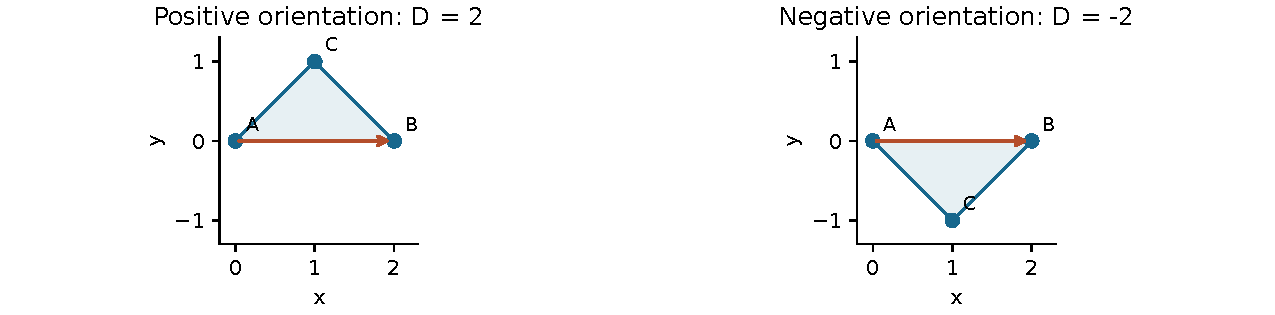
\includegraphics[width=0.92\linewidth]{figures/orientation_signs.pdf}
\end{center}

For $A=(0,0)$, $B=(2,0)$, and $C=(1,1)$, the determinant is $2$, so
the triangle has area one and positive orientation. Replacing $C$ by
$(1,-1)$ gives determinant $-2$. The magnitude measures area; many
algorithms need only the sign.

A \emph{geometric predicate} answers a discrete question such as which
side of a line contains a point. Its result may determine a branch in a
convex-hull, intersection, or triangulation algorithm. A small arithmetic
error near zero can therefore change the structure of the output, not just
the final digits of a coordinate. Computing accurate coordinates and
computing the correct branch decision are related but distinct tasks.

\begin{question}{Identify what has to be reliable}
Which sign changes when two points are exchanged? What happens if every
coordinate is multiplied by the same nonzero scale factor? Why might an
incorrect zero be more disruptive than a small relative error in a length?
\end{question}

We will specify exact rational input points, attempt a rigorous sign test
using ball arithmetic, and use exact rational arithmetic if needed. This
small filter is a teaching example. It does not implement the expansion
arithmetic used in Shewchuk's adaptive predicates, nor does one correct
predicate prove a whole geometry algorithm correct.

\newpage
\heading{2. Exactly represented inputs can still give a wrong zero}{13--29 minutes: a cancellation example with an exact reference}
Let $n=2^{27}$ and take
\[
 A=(0,0),\quad B=(n,n-1),\quad C=(n+1,n).
\]
Every coordinate is exactly representable in binary64. The exact determinant is
\[
                   n^2-(n-1)(n+1)=n^2-(n^2-1)=1.
\]
Nevertheless, ordinary binary64 multiplication and subtraction give zero.
The failure occurs after input representation: the two products round to
the same machine value before they are subtracted.
\begin{lstlisting}
from fractions import Fraction

def determinant(a, b, c):
    ab_x = b[0] - a[0]
    ab_y = b[1] - a[1]
    ac_x = c[0] - a[0]
    ac_y = c[1] - a[1]
    return ab_x * ac_y - ab_y * ac_x

n = 2**27
points = [(0, 0), (n, n-1), (n+1, n)]
float_points = []
exact_points = []
for x, y in points:
    float_points.append((float(x), float(y)))
    exact_points.append((Fraction(x), Fraction(y)))
assert determinant(*float_points) == 0.0
assert determinant(*exact_points) == 1
\end{lstlisting}

Why do the products coincide? The first is $n^2=2^{54}$, exactly
representable. Immediately below that value, adjacent binary64 numbers
are spaced by two. The integer $2^{54}-1$ is halfway between
$2^{54}-2$ and $2^{54}$; round-to-nearest with ties to even chooses
$2^{54}$. The final subtraction is exact for its stored operands, but
the information distinguishing the two original products has already vanished.

\textbf{An arbitrary zero tolerance changes the question.} A rule such as
``declare collinear if $|D|<10^{-10}$'' defines a tolerance-based notion,
not exact collinearity. Scaling all coordinates by $s\ne0$ multiplies $D$
by $s^2$ without changing its sign. Thus the same geometric configuration
in different units can cross a fixed determinant threshold. A physical
distance tolerance requires its own stated model and normalization.

\begin{question}{Locate the lost information}
Would subtracting the already rounded products at higher precision recover
the exact answer? Which inputs and operations must be recomputed? Why does
the integer calculation provide a stronger reference than a plotted triangle?
\end{question}

Python integers avoid rounding in this example. Fractions extend the exact
reference to rational coordinates, including intended decimal strings.
The next step uses a less expensive enclosure when that already decides
the sign, reserving exact fallback for unresolved cases.

\newpage
\heading{3. A filter answers only when inclusion decides the sign}{29--46 minutes: an enclosure, an exact comparison, and four outcomes}
Suppose $D\in[l,u]$ is a valid determinant enclosure for the specified
points. If $l>0$, the exact sign is positive; if $u<0$, it is negative.
The singleton $[0,0]$ proves exact zero. Every other zero-containing
enclosure is inconclusive. In particular, $[0,\delta]$ for $\delta>0$
proves nonnegativity but does not distinguish a positive determinant from zero.
\begin{lstlisting}
from flint import arb, ctx, fmpq

def sign_of_bounds(lower, upper):
    if lower > 0:
        return 1
    if upper < 0:
        return -1
    if lower == upper == 0:
        return 0
    return None

def coordinate_ball(value):
    return arb(fmpq(value.numerator, value.denominator))

def determinant_bounds(points, bits):
    with ctx.workprec(bits):
        balls = []
        for x, y in points:
            balls.append((coordinate_ball(x), coordinate_ball(y)))
        result = determinant(*balls)
        if not result.is_finite():
            return None
        midpoint = result.mid().fmpq()
        radius = result.rad().fmpq()
        return midpoint - radius, midpoint + radius
\end{lstlisting}

The input coordinates here are exact \texttt{Fraction} objects. Each is
converted to a containing Arb ball. Arithmetic operations enclose the
determinant, and exact rational extraction of the stored midpoint and
radius provides bounds for the final comparison. The code returns no
finite bound if the arithmetic cannot supply one; it does not manufacture
a sign from a nonfinite result.

\textbf{The proof is composition plus order.} Each exact coordinate lies
in its input ball. Subtractions and products preserve inclusion, so their
final combination contains the exact determinant. A strict endpoint sign
then applies to every value in that enclosure, including the intended
determinant. No estimate of the determinant's relative error is needed.

\begin{question}{Read each possible result precisely}
Classify $[2,3]$, $[-3,-2]$, $[0,0]$, $[-1,1]$, and $[0,1]$.
Which bounds settle exact collinearity? Why must \texttt{None} remain
distinct from the integer zero in a program's control flow?
\end{question}

\reading{The \href{https://python-flint.readthedocs.io/en/latest/arb.html}{python-flint Arb API}
provides the ball operations and midpoint/radius extraction. As in Lecture 05,
rounded display strings are not the certificate's endpoints.}

\newpage
\heading{4. Increase precision, then fall back to the exact problem}{46--62 minutes: a short filter with a recorded history}
Try a finite sequence of precisions. Each attempt must start again from the
exact coordinates. Widening the precision of an old uncertain result cannot
recover information lost earlier. If no attempt proves a sign, rational
evaluation of this determinant settles the same exact input problem.
\begin{lstlisting}
def orientation(points, precisions=(24, 53, 100, 200)):
    if len(points) != 3:
        raise ValueError("Need three planar points")
    for point in points:
        if len(point) != 2:
            raise ValueError("Need two coordinates per point")
        for value in point:
            if not isinstance(value, Fraction):
                raise TypeError("Specify each coordinate as a Fraction")
    attempts = []
    for bits in precisions:
        bounds = determinant_bounds(points, bits)
        attempts.append((bits, bounds))
        if bounds is not None:
            sign = sign_of_bounds(*bounds)
            if sign is not None:
                return sign, "arb", attempts
    exact = determinant(*points)
    if exact > 0:
        sign = 1
    elif exact < 0:
        sign = -1
    else:
        sign = 0
    return sign, "fraction", attempts

sign, method, attempts = orientation(exact_points)
assert sign == 1
sign, method, attempts = orientation(exact_points, precisions=(24,))
assert sign == 1 and method == "fraction"
\end{lstlisting}

This interface deliberately requires already specified rational coordinates.
It cannot silently decide whether an incoming float means an intended
decimal measurement or the exact stored binary value. The next page makes
that distinction explicit. The arithmetic library is \texttt{python-flint};
none of these excerpts imports the course package \texttt{vc}.

For finite rational coordinates, additions and products remain rational, so
the fallback supplies an exact sign, including exact collinearity. Its cost
can grow with numerator and denominator sizes. The point of filtering is
to avoid paying that cost when a less expensive valid bound already decides.
No performance superiority is claimed for this small teaching implementation.

\begin{question}{Audit the precision history}
Print the attempted bounds for the cancellation example. Which first
excludes zero? If the initial precision budget ends, why is exact fallback
legitimate here? What mathematical inputs must remain unchanged between attempts?
\end{question}

This construction is different from assuming a high-precision sign is
correct because it stops changing. Every accepted approximate-arithmetic
decision has an enclosing bound; the fallback has an exact rational value.

\newpage
\heading{5. State which geometric input is being certified}{62--77 minutes: decimal intent, stored floats, and measured families}
Compare $A=(0,0)$, $C=(10,1)$, and two interpretations of $B=(1,0.1)$.
If the second coordinate means the exact decimal $1/10$, the determinant
is $1-10(1/10)=0$. If it means the exact value of the stored binary64
number \texttt{0.1}, that value is slightly larger, so the determinant
is negative. Both decisions can be correct because the inputs differ.
\begin{lstlisting}
a = (Fraction(0), Fraction(0))
c = (Fraction(10), Fraction(1))
decimal_b = (Fraction(1), Fraction("0.1"))
stored_b = (Fraction(1), Fraction.from_float(0.1))
assert determinant(a, decimal_b, c) == 0
assert determinant(a, stored_b, c) == Fraction(-1, 2**54)
assert orientation([a, decimal_b, c])[0] == 0
assert orientation([a, stored_b, c])[0] == -1
\end{lstlisting}

The exact fallback does not recover the user's decimal intention from a
binary float. It solves precisely the rational problem it is given. Input
interpretation therefore belongs in a geometric certificate alongside its
arithmetic evidence.

\textbf{Measurements describe a family.} Now take $A=(0,0)$, $B=(1,1)$,
and let $C=(2,y)$ with $y\in[1.999,2.001]$. The determinant is $y-2$,
so its exact range is $[-1/1000,1/1000]$. The two allowed endpoint
realizations have opposite signs, and the midpoint realization is collinear.
There is no single orientation valid for every member of this family.

Increasing arithmetic precision cannot resolve that physical ambiguity.
Replacing $y$ by its midpoint and calling the exact-point filter would
answer a different question. Instead, an interval-coordinate evaluator
must retain the full measurement sets and report that a uniform sign
has not been established.

\begin{question}{Distinguish two reasons for an undecided sign}
A zero-containing arithmetic enclosure for one exact point triple may be
too wide. A measured family may genuinely allow both signs. What evidence
distinguishes these situations? Does a zero-containing enclosure alone prove
that both orientations actually occur?
\end{question}

The last question matters when coordinates are correlated. Independent
coordinate boxes may include combinations ruled out by a physical relation.
Their determinant enclosure remains valid for the admissible subset, but
extra signs in the enclosure may be artifacts of that relaxation. In our
example, the two explicit admissible realizations prove real ambiguity.

\textbf{A correct report.} For exact inputs, state the sign and its
arithmetic evidence. For uncertain inputs, state a determinant enclosure
and whether it proves one sign for the whole family. If it does not, retain
the uncertainty in any downstream branch decision instead of silently
substituting a representative configuration.

\newpage
\heading{6. Exercises and the bridge to collision decisions}{77--90 minutes: choose two exercises and audit an application claim}
\begin{enumerate}
\item \textbf{Area, order, and scale.} Compute the determinant for
$(0,0),(3,0),(1,2)$ and the triangle's area. Exchange the last two points,
then scale all coordinates by $1/1000$. Explain why orientation is unchanged
by the common scaling although a fixed determinant tolerance may change
its classification.

\item \textbf{Exact zero versus unresolved.} Classify the five bounds
on page 3. Use exact fractions to show that $(0,0),(1/3,2/3),(2/3,4/3)$
are collinear. If Arb returns an interval straddling zero for these inputs,
is the mathematical answer uncertain or merely the current arithmetic test?

\item \textbf{Two different input specifications.} Reproduce the decimal
and stored-float example. Explain why converting the stored tenth to a
100-digit nearest-rounded number cannot make its exact determinant zero.
State what must change to solve the intended-decimal problem instead.

\item \textbf{A proper segment crossing.} For segments $AB$ and $CD$,
strictly opposite signs of $D(A,B,C)$ and $D(A,B,D)$, together with
strictly opposite signs of $D(C,D,A)$ and $D(C,D,B)$, certify a proper
interior crossing. Check this for $A=(0,0)$, $B=(2,2)$, $C=(0,2)$,
$D=(2,0)$. Why do zero orientations require additional handling of
collinearity, endpoint contact, and whether projected intervals overlap?

\item \textbf{Order collision times.} Candidate first-hit times satisfy
$t_1\in[1,11/10]$ and $t_2\in[21/20,6/5]$. Can these bounds alone prove
which event occurs first? State a sufficient endpoint inequality for
ordering two time enclosures. Why is reflecting from the midpoint-selected
mirror insufficient for a validated trajectory?
\end{enumerate}

\textbf{Selected checks.} Exercise 1: $D=6$, area $3$; swapping gives
$-6$ and common scaling multiplies the determinant by $10^{-6}$.
Exercise 2: positive, negative, zero, inconclusive, inconclusive, respectively.
The rational collinearity determinant is exactly zero. Exercise 3: the
stored-input determinant is $-1/2^{54}$; a different precision does not
change the specified real input. Exercise 4: the four determinants are
$4,-4,-4,4$. Exercise 5: the time intervals overlap, so either ordering
is compatible with those bounds alone; $\sup T_1<\inf T_2$ would prove
the first candidate earlier.

\begin{question}{Exit ticket: a predicate is one part of a proof}
Distinguish exact collinearity, an inconclusive arithmetic bound, and a
family admitting several orientations. Then identify one further condition
needed by a segment-intersection algorithm or a first-collision simulation.
\end{question}

The mirror capstone also needs existence of the proposed collision,
exclusion of earlier events, appropriate treatment of grazing or simultaneous
hits, and a valid reflection update. A correct sign filter supplies a
building block for those arguments, not a certificate for an entire trajectory.

\reading{Companion: \texttt{notebooks/12\_robust\_geometry.ipynb} and Lab 12.
\href{https://www.cs.cmu.edu/~quake/robust.html}{Shewchuk, \emph{Adaptive Precision Floating-Point Arithmetic and Fast Robust Geometric Predicates} (1997)}.
Our filter uses Arb and rational fallback. Next: certificate audit and the
mirror-trajectory project.}
\end{document}
